\documentclass{article}

\usepackage[final]{neurips_2026}
\usepackage[utf8]{inputenc}
\usepackage[T1]{fontenc}
\usepackage{hyperref}
\usepackage{url}
\usepackage{booktabs}
\usepackage{amsmath}
\usepackage{graphicx}
\usepackage{flafter}
\usepackage{placeins}
%\usepackage{microtype}
\usepackage{xcolor}

\setcitestyle{authoryear,round}

\title{Same Persona, Different Language, Different Deal: Cross-Lingual Effects in LLM Negotiation}
\workshoptitle{SocialAgent: Second Workshop on Large Language Models for Social Reasoning and Simulation}
\author{%
  Saehee Eom \\
  Georgia Institute of Technology \\
  \texttt{seom@gatech.edu} \\
  \And
  Tejas Khandwekar \\
  Georgia Institute of Technology \\
  \texttt{tkhandwekar3@gatech.edu} \\
}

\begin{document}
\maketitle

\begin{abstract}
Tell an LLM negotiator to be ``headstrong'' and it should hold firm on
price, but does that instruction retain the same behavior in every language? To test this, we use identical buyer and seller instances of Gemini 3.6 Flash
to negotiate the same 12 CraigslistBargain scenarios in English and Korean.
The pilot-scale $2\times2\times3$ design crosses interaction language, seller
urgency (none or strong), and buyer persona (cooperative, neutral, or
headstrong), yielding 432 attempted negotiations. We call this property \emph{cross-lingual
social-policy fidelity}: whether a prompt-defined social policy produces the
same behavioral effect regardless of interaction language. It often does
not. Korean negotiations reached agreement far more often than English
(77.3\% vs.\ 52.5\%, a 24.8-point gap, Holm-adjusted $p=.0039$), but only for
neutral and headstrong buyers; cooperative buyers were already near-ceiling
in both languages. Buyers' opening offers barely differed by language; the
gap instead emerged later, through larger seller concessions and a smaller
final gap in Korean, and agreed prices were also lower in Korean. This
language effect is not an artifact of a single model: repeating the full
negotiation with Qwen3 as both agents reproduces the same direction of
effect on both agreement rate ($+13.9$pp Korean vs.\ Gemini's $+24.8$pp) and
conditional final price ($-18.8$pp vs.\ $-25.0$pp), smaller in magnitude but
consistent in sign. Another model labeled every turn for face-threatening acts and
politeness-mitigation strategy: Korean dialogue showed consistently higher
mitigation, most sharply for sellers (11.7\% vs.\ 3.6\% of face-threatening
turns), and a higher share of positive-politeness strategies. These results show that such a policy can produce
different simulated negotiation behavior, not just different wording, when only the
interaction language changes. This shift holds across at least two
different underlying models.
\end{abstract}

\section{Introduction}
Negotiation is a compact test of socially situated agents: models must track
goals, read counterparts, choose offers, and decide whether to concede,
accept, or walk away. Early neural negotiators learned strategy and language
jointly \citep{lewis2017deal}; CraigslistBargain later decoupled them through
grounded buyer--seller dialogue acts \citep{he2018decoupling}. Recent LLM work
shows that tactics, roles, personality, and social framing also affect
negotiation outcomes \citep{bianchi2024negotiationarena,kwon2024negotiators,
xia2024bargaining,huang2024personality,noh2026personalities,vaccaro2026advancing}.


Language itself shapes negotiation outcomes: multilingual studies find that
agreement rates, stability, and reasoning behavior all shift with the
language used \citep{sinha2026language,hakimov2026price}, and prompt
politeness and social reasoning vary across languages, Korean included
\citep{yin2024respect,jung2024koreanpoliteness,kim2026socialreasoning}.
Yet language and social configuration are almost always studied separately,
leaving an open question for deployment: does a persona, or a response to a
counterpart's hardship, still work the same way once the interaction
language changes?

We answer this question with matched English--Korean self-play: the same 12
items, private targets, bargaining rules, model, and
decoding settings, crossed only with seller urgency and buyer persona.
Because every turn carries both an utterance and a structured action, we do
not have to infer strategy from the text. We can see exactly where anchors,
concessions, and the final buyer--seller gap actually move. We call this
target property \textbf{cross-lingual social-policy fidelity}: whether a
persona or hardship based policy keeps its behavioral effect across interaction
languages.

We evaluate cross-lingual social-policy fidelity at two levels. Structured
actions reveal where agreement, concessions, and terminal gaps diverge, while
a separate judge model characterizes face-threatening acts (FTAs), mitigation,
and politeness strategies across languages. These pragmatic annotations are secondary, descriptive evidence and do not establish a causal mechanism.

\section{Method}
\label{sec:method}

\subsection{Experimental design and procedure}

We sampled 12 CraigslistBargain scenarios from the Stanford NLP distribution
\citep{he2018decoupling,stanfordnlp2026craigslist}, two from each of six
categories (housing, furniture, cars, bikes, phones, and electronics), using
seed 42. Each scenario contains a listing price and private buyer and seller
targets. Korean titles and descriptions were machine translated and manually checked
(translation QA details in Appendix~\ref{app:reproducibility}). U.S. locations and dollar prices were
deliberately retained, so the Korean condition is a translated U.S.
marketplace setting, not a localized Korean market.
We crossed language $\{\mathrm{English},\mathrm{Korean}\}$,
seller urgency $\{\mathrm{none},\mathrm{strong\ need\ for\ cash}\}$, and buyer
persona $\{\mathrm{cooperative},\mathrm{neutral},\mathrm{headstrong}\}$ in a
full factorial design. The cooperative prompt aims for a workable deal and
concedes readily; the headstrong prompt anchors on the target and concedes
slowly; neutral adds no disposition. Urgency appears only in the seller
prompt and persona only in the buyer prompt. We ran every condition three
times on every scenario: $12\times 12\times 3=432$ attempted negotiations.

Buyer and seller were separate instances of \texttt{gemini-3.6-flash} at temperature 0.2. The seller opened at the listing price;
roles then alternated for at most 16 turns. Each response had to contain an
utterance, an action in \{offer, counter-offer, accept, reject\}, and an
optional price. An accept ended in \texttt{agreed}, an explicit terminal
reject in \texttt{abandoned}, and exhausting all 16 turns in
\texttt{max\_turns\_reached}. Two negotiations failed semantic parsing after three attempts and were
excluded without replacement; both were English/strong/headstrong. Thus 430 negotiations and 4,580 valid turns entered analysis:
279 agreements, 118 abandonments, and 33 turn-cap outcomes.

\subsection{Measures and pragmatic annotation}

Primary outcomes are agreement, the three-way outcome mode
(\texttt{agreed} /  \texttt{abandoned} /  \texttt{max\_turns\_reached}), turns,
turn-cap rate, and agreed price. Agreement rate and price achieved match
prior LLM benchmarking on CraigslistBargain \citep{agreemate2024} for
comparability. To compare heterogeneous dollar scales, we normalize price as
$z(p)=(p-\text{buyer target})/(\text{seller target}-\text{buyer target})$,
so 0 is the buyer target and 1 the seller target; values are not clipped.
Agreed-price analyses exclude failed negotiations and are conditional on
reaching agreement. Process measures track opening offers, role-specific concessions, normalized
offer trajectories, and the final buyer--seller gap, including failed
negotiations.

A separate model, \texttt{qwen/qwen3.7-flash}, labeled each valid turn for
face-threatening acts (FTAs) using Brown--Levinson politeness
strategies \citep{brown1987politeness,dutt2020face}. We additionally interpret
language differences through Ting-Toomey's Face-Negotiation Theory
\citep{tingtoomey1985conflict}. These judge-derived measures characterize pragmatic style without testing
mediation.


\subsection{Statistical analysis}

For each scenario, we average the three repetitions within each factorial cell
and then across the 12 scenarios so that each scenario contributes equally.
Confidence intervals use 10,000 scenario-block bootstrap samples (seed 42).
Four prespecified agreement contrasts were tested with exact, two-sided
sign-flip tests: the language main effect, language$\times$urgency,
language$\times$(cooperative$-$neutral), and
language$\times$(headstrong$-$neutral). Holm correction was applied across
these four tests; other effects are exploratory.

\section{Results}
\label{sec:results}

\subsection{Agreement outcomes}

Scenario-balanced agreement was 52.5\% in English (112/214 valid runs) and
77.3\% in Korean (167/216), a $+24.8$-point contrast (Table~\ref{tab:headline};
full per-cell counts are in Appendix~\ref{app:cells}, and per-scenario
counts in Appendix~\ref{app:scenario-agreement}).
Strong seller urgency also raised agreement from 50.0\% to 79.9\%
($+29.9$ points). The $+16.2$-point language$\times$urgency contrast has a
bootstrap interval above zero, but its exact test does not survive the
four-test Holm family ($p=.1133$).


\begin{figure}[t]
  \centering
  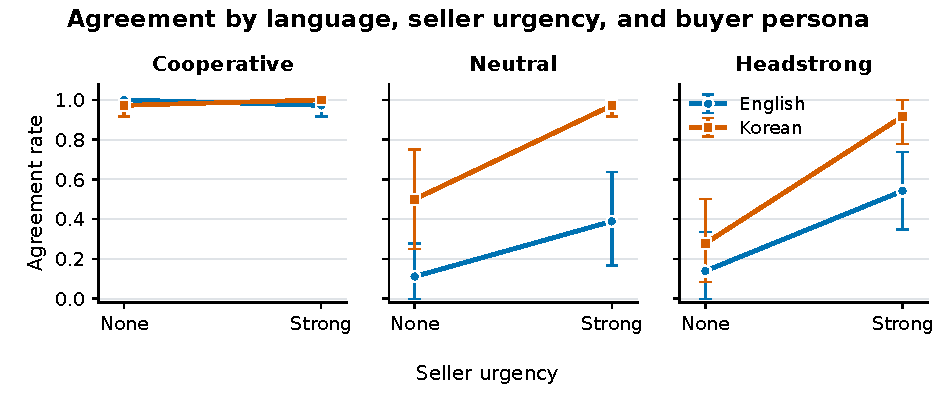
\includegraphics[width=.85\linewidth]{figures/agreement_interactions.pdf}
  \caption{Scenario-balanced agreement by language, seller urgency, and buyer
  persona; bars are 95\% scenario-block bootstrap intervals. Cooperative
  agreement is near ceiling in both languages, while Korean most strongly
  changes neutral and headstrong outcomes.}
  \label{fig:agreement}
\end{figure}

The language contrast is not uniform across personas
(Figure~\ref{fig:agreement}). Cooperative buyers reached 98.6\% agreement in
both languages, leaving no room for a language gain. Neutral agreement rose
from 25.0\% in English to 73.6\% in Korean; headstrong agreement rose from
34.0\% to 59.7\%. Accordingly, both language-by-persona contrasts were
confirmed after Holm correction. Exploratory three-way intervals crossed
zero, so urgency does not clearly modify these language-by-persona
differences further.

\begin{table}[t]
\caption{Scenario-balanced agreement contrasts. Estimates are percentage
points; intervals use 10,000 scenario-block bootstraps. Holm $p$ values apply
only to the four prespecified exact tests. All rows use 430 valid runs, 279
agreements, and 12 scenarios.}
\label{tab:headline}
\centering
\small

\begin{tabular}{lrrr}
\toprule
Contrast & Estimate & 95\% CI & Adjusted $p$ \\
\midrule
Korean $-$ English & $24.8$ & $[15.7,34.7]$ & $.0039$ \\
Strong urgency $-$ none & $29.9$ & $[20.1,39.6]$ & n/a \\
Language $\times$ urgency & $+16.2$ & $[0.9,32.9]$ & $.1133$ \\
Language $\times$ (cooperative $-$ neutral) & $-48.6$ & $[-66.7,-30.6]$ & $.0039$ \\
Language $\times$ (headstrong $-$ neutral) & $-22.9$ & $[-36.8,-8.3]$ & $.0391$ \\
\bottomrule
\end{tabular}
\end{table}


\subsection{Negotiation dynamics and agreed prices}

The normalized first buyer offer differed by only $+0.024$ in Korean (95\% CI
$[-0.011,0.056]$). Later behavior diverged: Korean reduced buyer net
concession by $0.086$ target spans (CI $[-0.137,-0.041]$), increased seller
net concession by $0.349$ spans (CI $[0.237,0.462]$), and reduced the
terminal buyer--seller gap by $0.286$ spans (CI $[-0.400,-0.175]$). Thus the
agreement result is more consistent with different concession dynamics and
gap closure than with a different buyer opening anchor. Mean length differed
by only $+0.41$ turns (CI $[-0.17,1.07]$), while strong urgency shortened
negotiations by $0.94$ turns (CI $[-1.58,-0.33]$). Full offer trajectories are in Appendix~\ref{app:trajectories}. Among 279 agreements, normalized price averaged 0.513 in English and 0.263
in Korean, a $-0.250$ contrast (CI $[-0.315,-0.178]$), favoring buyers. This
gap does not mean Korean negotiations produce better prices for buyers in
general: language changes which negotiations reach agreement, and only two
scenarios supplied agreements in every full factorial cell. We therefore use
price only to describe the selected agreement set.

\subsection{Robustness to a second negotiator model}
We repeated the full design with Qwen3 as both agents
(Appendix~\ref{app:qwen-validation}). The Korean advantage replicated in
direction for agreement ($+13.9$ vs.\ Gemini's $+24.8$ points) and conditional
price ($-18.8$ vs.\ $-25.0$ points), with smaller but consistent effects.
We read this as descriptive robustness rather than a third confirmatory test.

\subsection{Politeness and pragmatic annotations}
FTA rates were high and similar across languages, unsurprisingly, since
rejecting an offer or countering a price is itself face-threatening. What
differed was mitigation: Korean turns softened the face threat notably more
often than English, most sharply for sellers. Korean dialogue also used a
higher share of positive-politeness strategies for both roles (full rates
and strategy composition by role are in Appendix~\ref{app:pragmatics}).
These labels are compatible with a language-conditioned realization
difference, but neither their observational association with agreement nor
a judge-model label establishes a mechanism.


\section{Discussion}
\label{sec:discussion}

The 24.8-point Korean gain is not uniform across buyer types. Neutral and headstrong buyers drive it, while cooperative buyers were already near ceiling. This divergence appears only after the opening offer, as sellers concede further and the two sides end up closer together in Korean. This matches the failure
mode cross-lingual social-policy fidelity predicts: the persona's wording
stays the same across languages, but its economic effect does not.

The language effect is concentrated in abandonment rather than the turn cap:
English had 39.1\% abandonment versus 15.7\% in Korean. Strong urgency independently increased agreement, but its interaction with
language remained only suggestive (Table~\ref{tab:headline}). All inferential tests treat the 12 scenarios, not the 430 runs, as
independent units. A matched second-model validation preserved the Korean-language direction in
agreement and the same seller-concession and gap-closure pattern
(Appendix~\ref{app:qwen-validation}).This evaluation is useful because it makes a deployable failure
visible before an agent represents real users: teams
can check whether persona and hardship policies stay behaviorally stable
across the languages they support. The same instability could give users different deals or prices depending
on their interface language; higher agreement is not automatically fairer or
better for users. The experiment must not be used to
stereotype human negotiators; it measures model behavior under translated
prompts. Any deployment audit should report agreement alongside selection into
observed prices and role-specific concessions, not agreement alone.

\section{Limitations and future work}
\label{sec:limitations}
This pilot covers 12 scenarios, three repetitions, and one primary model, using translated rather than localized Korean materials. Part of the persona/urgency prompt effects could come from translation strength. Qwen3 directionally supports the outcome and offer-process findings but was not scored for pragmatic annotations
(Appendix~\ref{app:qwen-validation}). The politeness labels were generated by an LLM judge without formal human validation, so we treat them as descriptive. Conditional prices remain selected on
agreement, and pragmatic labels received qualitative rather than formal human
calibration. Future work should test additional models, languages, localized
markets, and human-calibrated pragmatics. Reproducibility and exclusion details
are in Appendix~\ref{app:reproducibility}.
\clearpage

\bibliographystyle{plainnat}
{\small
\bibliography{references}
}


\clearpage
\appendix

\section{Agreement outcomes by scenario}
\label{app:scenario-agreement}

Table~\ref{tab:scenario-agreement} reports agreement separately for each
scenario and interaction language. Rates average the factorial conditions and
repetitions available within a scenario.

\begin{table}[ht]
\caption{Agreement by scenario and interaction language. $A/N$ denotes
agreements per valid negotiation. The difference is the Korean-language rate
minus the English-language rate in percentage points. The summary row reports
total counts and scenario-balanced rates.}
\label{tab:scenario-agreement}
\centering
\small
\begin{tabular}{llrrrrr}
\toprule
& & \multicolumn{2}{c}{English} & \multicolumn{2}{c}{Korean} & \\
\cmidrule(lr){3-4}\cmidrule(lr){5-6}
Scenario & Category & $A/N$ & Rate (\%) & $A/N$ & Rate (\%) & Difference \\
\midrule
00 & Furniture   & 9/17  & 52.9  & 12/18 & 66.7  & 13.7 \\
01 & Car         & 8/18  & 44.4  & 16/18 & 88.9  & 44.4 \\
02 & Bike        & 5/18  & 27.8  & 10/18 & 55.6  & 27.8 \\
03 & Phone       & 6/18  & 33.3  & 17/18 & 94.4  & 61.1 \\
04 & Bike        & 7/18  & 38.9  & 9/18  & 50.0  & 11.1 \\
05 & Electronics & 10/18 & 55.6  & 15/18 & 83.3  & 27.8 \\
06 & Car         & 7/17  & 41.2  & 12/18 & 66.7  & 25.5 \\
07 & Housing     & 12/18 & 66.7  & 14/18 & 77.8  & 11.1 \\
08 & Phone       & 13/18 & 72.2  & 17/18 & 94.4  & 22.2 \\
09 & Electronics & 18/18 & 100.0 & 18/18 & 100.0 & 0.0 \\
10 & Furniture   & 7/18  & 38.9  & 15/18 & 83.3  & 44.4 \\
11 & Housing     & 10/18 & 55.6  & 12/18 & 66.7  & 11.1 \\
\midrule
Summary & & 112/214 & 52.5 & 167/216 & 77.3 & 24.8 \\
\bottomrule
\end{tabular}
\end{table}


\FloatBarrier

\section{Full outcome cells}
\label{app:cells}

Table~\ref{tab:cells} keeps abandonment and the 16-turn cap separate. Price is
normalized and conditional on agreement. The two technical exclusions are in
English/strong/headstrong.

\begin{table}[ht]
\caption{Full factorial outcomes. $A/V$ is attempted/valid; $D$, $B$, and $C$
are deal, abandonment, and cap rates. $z(p)$ is conditional on the listed
number of agreements. Every row contains 12 scenarios.}
\label{tab:cells}
\centering
\small
\begin{tabular}{lllrrrrr}
\toprule
Lang. & Urgency & Persona & $A/V$ & $D$ & $B$ & $C$ & $z(p)$ ($n$) \\
\midrule
EN & none & cooperative & 36/36 & 1.000 & 0.000 & 0.000 & .939 (36) \\
EN & none & neutral     & 36/36 & .111 & .889 & 0.000 & .270 (4) \\
EN & none & headstrong  & 36/36 & .139 & .583 & .278 & .705 (5) \\
EN & strong & cooperative & 36/36 & .972 & .028 & 0.000 & .751 (35) \\
EN & strong & neutral     & 36/36 & .389 & .611 & 0.000 & .092 (14) \\
EN & strong & headstrong  & 36/34 & .542 & .236 & .222 & .320 (18) \\
KO & none & cooperative & 36/36 & .972 & 0.000 & .028 & .704 (35) \\
KO & none & neutral     & 36/36 & .500 & .472 & .028 & .251 (18) \\
KO & none & headstrong  & 36/36 & .278 & .444 & .278 & .122 (10) \\
KO & strong & cooperative & 36/36 & 1.000 & 0.000 & 0.000 & .428 (36) \\
KO & strong & neutral     & 36/36 & .972 & .028 & 0.000 & .040 (35) \\
KO & strong & headstrong  & 36/36 & .917 & 0.000 & .083 & .034 (33) \\
\bottomrule
\end{tabular}
\end{table}

\FloatBarrier

\section{Offer trajectories}
\label{app:trajectories}
\begin{figure}[ht]
  \centering
  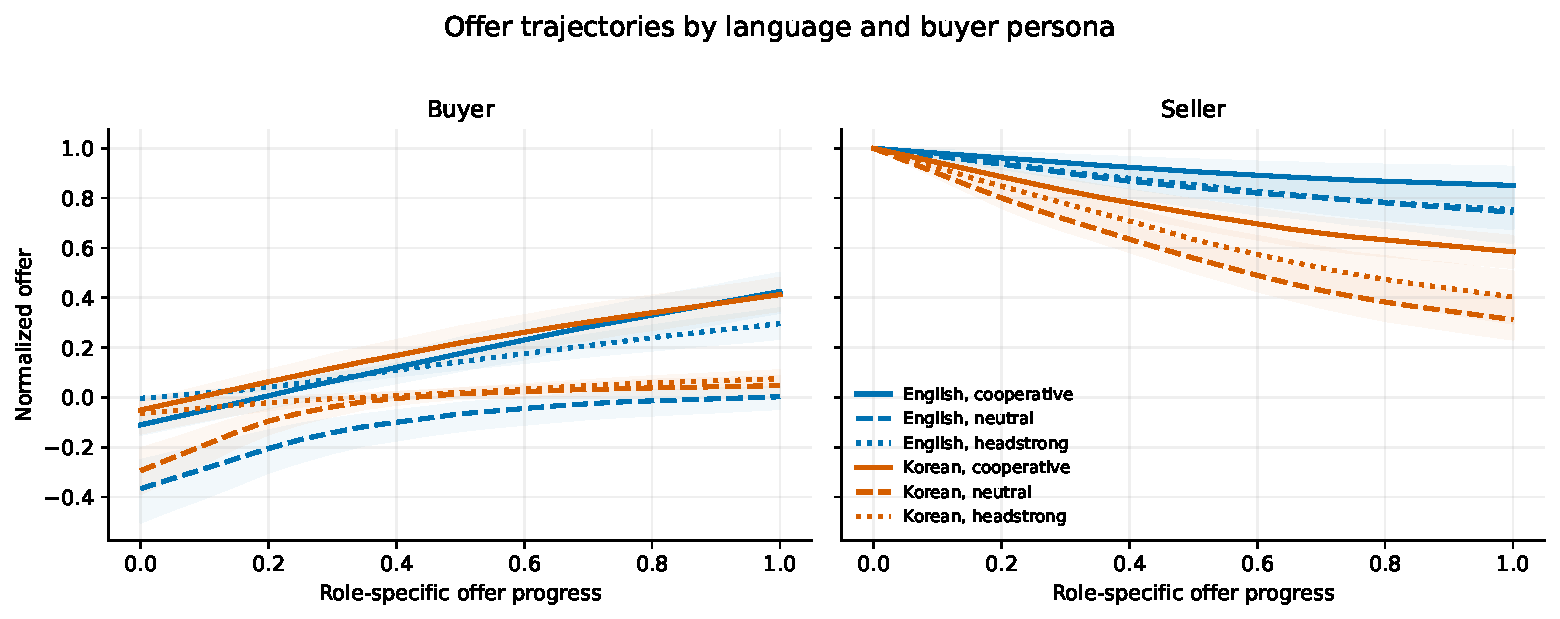
\includegraphics[width=.9\linewidth]{figures/offer_trajectories_language_persona.pdf}
  \caption{Normalized buyer and seller offers over negotiation progress,
  aggregated with equal scenario weight. Trajectories are descriptive because
  negotiations end at different times and for different reasons.}
  \label{fig:trajectories}
\end{figure}

\FloatBarrier

\section{Second-model validation}
\label{app:qwen-validation}


We repeated the complete $2\times2\times3$ design with
\texttt{qwen/qwen3.7-flash} as both buyer and seller, routed through OpenRouter
at temperature 0.2. 
The only change from the primary experiment was the negotiator model. The 12 scenarios, English and Korean materials, social policy prompts, private target values, three repetitions, role order, and 16-turn stopping rule all stayed the same.
All 432 planned Qwen negotiations were
present and parsable: 180 ended in agreement, 237 in abandonment, and 15 at
the turn limit. 
Because this validation set has no pragmatic judge labels, the
comparison is limited to terminal outcomes and structured offers.

Agreement was 34.7\% in the English condition (75/216) and 48.6\% in the
Korean condition (105/216), a scenario-balanced increase of 13.9 percentage
points (Table~\ref{tab:qwen-validation}). Strong seller urgency also retained
a large association with agreement, increasing it by 44.4 points. The Korean
condition had higher agreement within every buyer persona: 63.9\% versus
48.6\% for cooperative buyers, 36.1\% versus 22.2\% for neutral buyers, and
45.8\% versus 33.3\% for headstrong buyers. Qwen distributed the language
contrast more evenly across personas than Gemini, indicating that the exact
size of persona-specific contrasts varies across model families.

\begin{table}[ht]
\caption{Scenario-balanced estimates from the Qwen validation. Language
contrasts are Korean minus English; the urgency contrast is strong minus none.
Agreement and urgency use all 432 runs, while offer-process rows use the 425
runs with analyzable price-bearing sequences. Every row covers 12 scenarios.}
\label{tab:qwen-validation}
\centering
\small
\begin{tabular}{lrr}
\toprule
Contrast & Estimate & 95\% CI \\
\midrule
Agreement (percentage points) & $+13.9$ & $[0.0,28.7]$ \\
Strong seller urgency (percentage points) & $+44.4$ & $[37.5,51.4]$ \\
First buyer offer & $+0.017$ & $[-0.004,0.038]$ \\
Buyer net concession & $+0.009$ & $[-0.018,0.033]$ \\
Seller net concession & $+0.121$ & $[0.031,0.222]$ \\
Terminal buyer-seller gap & $-0.147$ & $[-0.235,-0.065]$ \\
\bottomrule
\end{tabular}
\end{table}

\begin{figure}[ht]
  \centering
  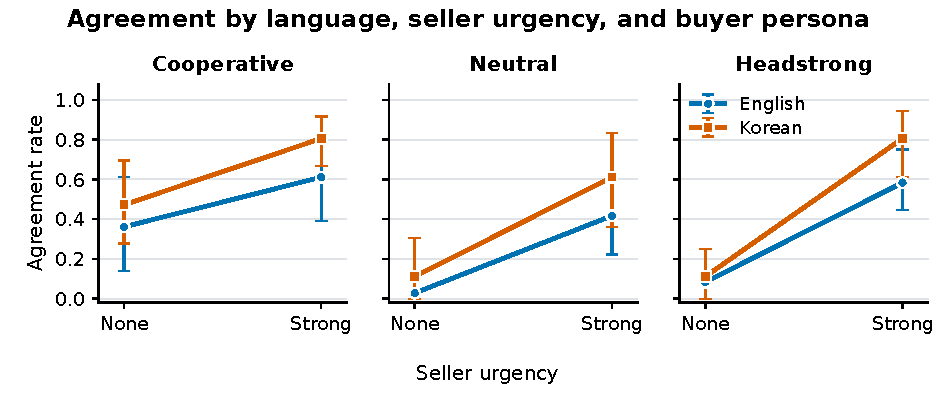
\includegraphics[width=\linewidth]{figures/agreement_interactions_qwen.pdf}
  \caption{Scenario-balanced Qwen agreement by language, seller urgency, and
  buyer persona across all 432 assigned-condition runs. Error bars show 95\%
  scenario-block bootstrap intervals.}
  \label{fig:qwen-agreement}
\end{figure}

The offer data show the same process signature as the primary experiment.
Buyer opening anchors remained similar across languages, while sellers in the
Korean condition made larger net concessions and negotiations ended with
smaller buyer-seller gaps. Figure~\ref{fig:qwen-trajectories} shows that this
pattern develops over the course of the negotiation rather than at the opening
anchor.

\begin{figure}[ht]
  \centering
  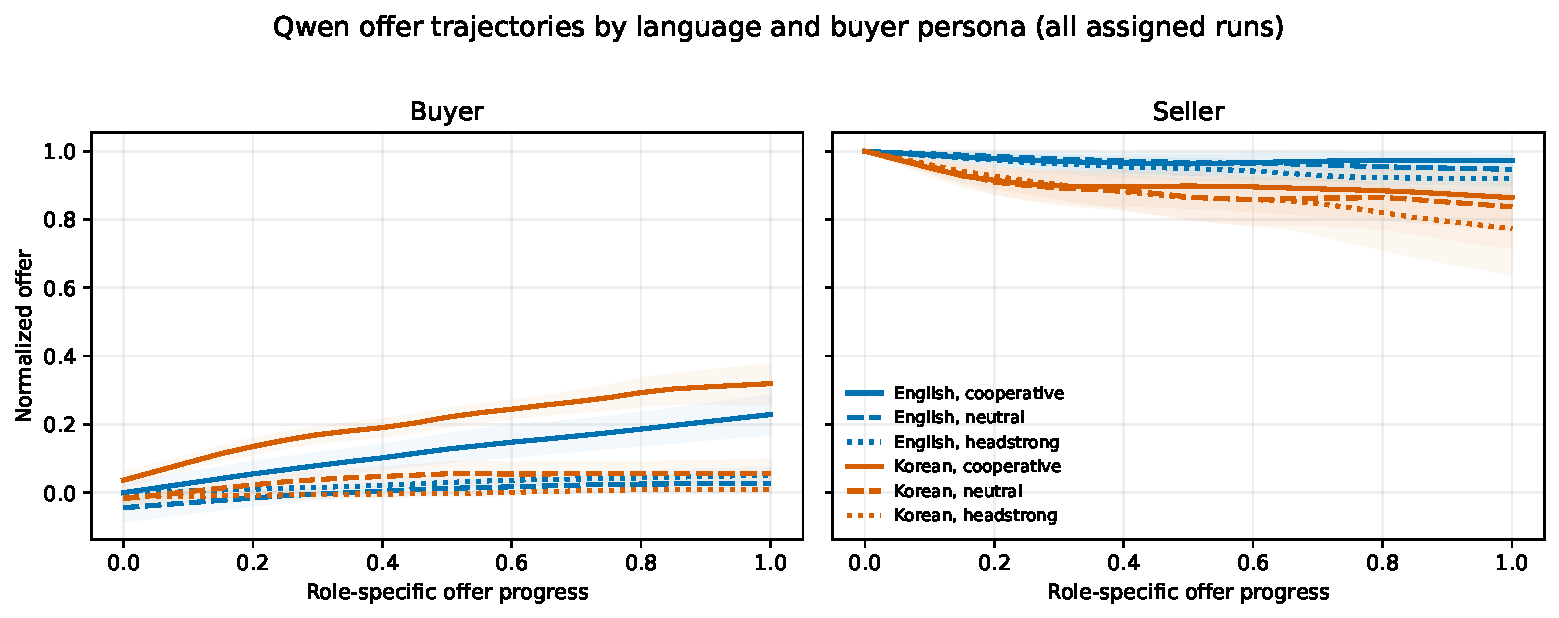
\includegraphics[width=.9\linewidth]{figures/offer_trajectories_language_persona_qwen.pdf}
  \caption{Normalized Qwen buyer and seller offers over negotiation progress,
  aggregated with equal scenario weight. The figure includes 425 runs with
  analyzable offer sequences; seven one-turn acceptances contained no offer
  trajectory.}
  \label{fig:qwen-trajectories}
\end{figure}

Twelve Korean-condition runs produced English-only dialogue. Excluding these
runs left the agreement contrast unchanged at $+13.9$ points, and a
conservative schema-compliant sensitivity estimate was $+14.4$ points. The
direction therefore holds across the full analysis and
both sensitivity checks. We reserve the cross-model confirmation for
agreement and offer-process outcomes because no Qwen scenario supplied
agreements in every factorial cell needed for an equally weighted conditional
price contrast.

\FloatBarrier

\section{Pragmatic summaries}
\label{app:pragmatics}

\begin{figure}[ht]
  \centering
  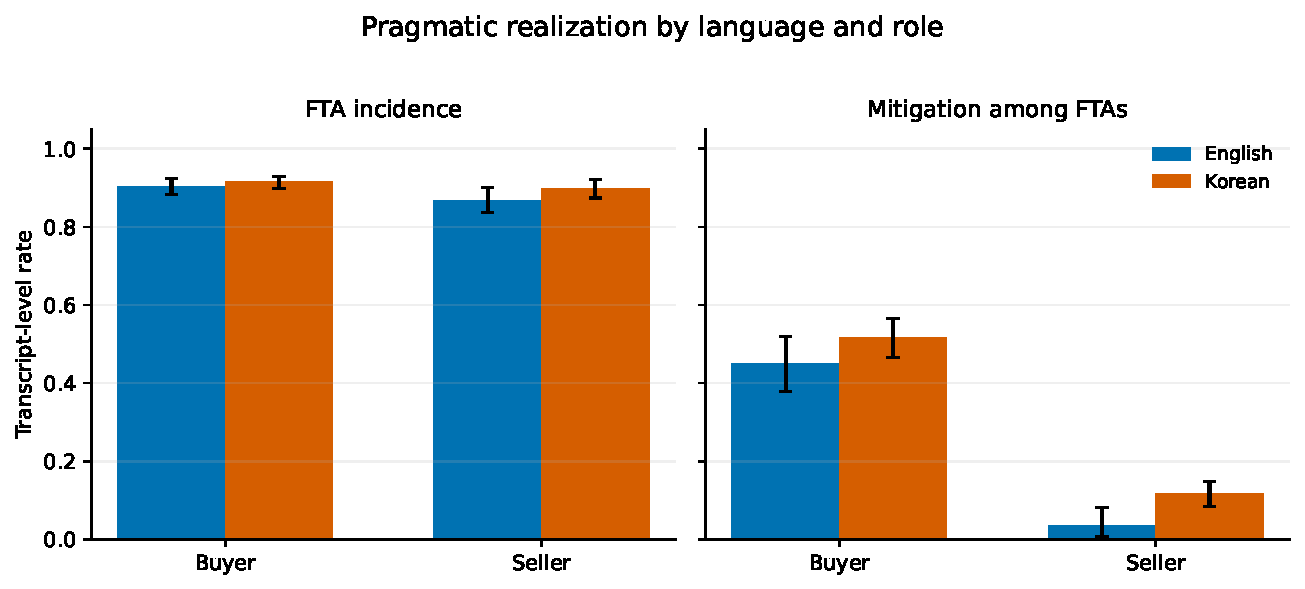
\includegraphics[width=.78\linewidth]{figures/pragmatic_rates_language_role.pdf}
  \caption{Transcript-level FTA and mitigation rates by language and role.
  Bars are 95\% scenario-block bootstrap intervals. These judge-derived
  measures are descriptive and are not used for causal mediation.}
  \label{fig:pragmatics}
\end{figure}

\begin{table}[ht]
\caption{Judge-derived pragmatic rates. Counts are valid transcripts; all rows
cover 12 scenarios. Mitigation is conditional on judge-labeled FTAs.}
\label{tab:pragmatics}
\centering
\small
\begin{tabular}{llrrrr}
\toprule
Language & Role & Runs & Agreements & FTA rate & Mitigation rate \\
\midrule
English & buyer  & 214 & 112 & .904 & .449 \\
Korean  & buyer  & 216 & 167 & .916 & .516 \\
English & seller & 214 & 112 & .868 & .036 \\
Korean  & seller & 216 & 167 & .899 & .117 \\
\bottomrule
\end{tabular}
\end{table}

\begin{figure}[ht]
  \centering
  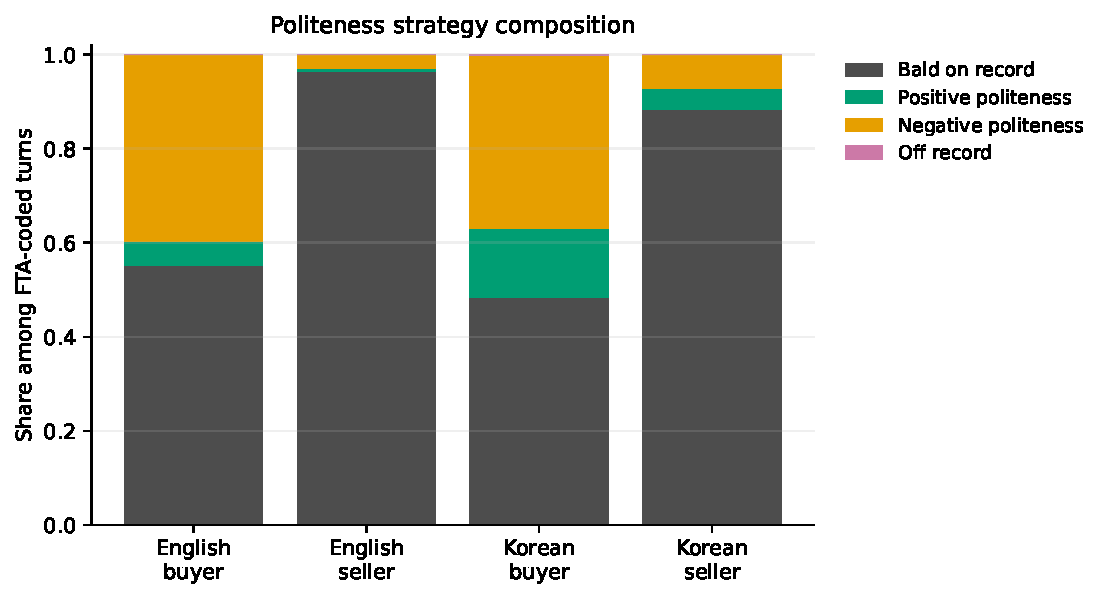
\includegraphics[width=.82\linewidth]{figures/politeness_strategy_composition.pdf}
  \caption{Composition of judge-labeled Brown and Levinson politeness
  strategies by interaction language and role. Shares are conditional on an
  FTA and are descriptive.}
  \label{fig:politeness-composition}
\end{figure}

\begin{table}[ht]
\caption{Scenario-balanced mean politeness-strategy shares among judge-labeled
FTAs.}
\label{tab:politeness-composition}
\centering
\small
\begin{tabular}{llrrrr}
\toprule
Language & Role & Bald & Positive & Negative & Off record \\
\midrule
English & buyer  & .551 & .053 & .396 & .000 \\
Korean  & buyer  & .484 & .146 & .369 & .002 \\
English & seller & .964 & .007 & .030 & .000 \\
Korean  & seller & .883 & .045 & .071 & .000 \\
\bottomrule
\end{tabular}
\end{table}

\FloatBarrier

\section{Model and API configuration}
\label{app:model-config}

Table~\ref{tab:model-config} reports the generation settings recoverable from
the collection code and stored outputs. Credentials and cloud-project
identifiers are omitted. The judge model slug is stored in every judged file;
the raw negotiation files do not serialize the negotiator model or API
settings.

\begin{table}[ht]
\caption{Recorded model and API configuration. Unspecified settings were not
passed by the code and therefore used provider defaults.}
\label{tab:model-config}
\centering
\small
\setlength{\tabcolsep}{4pt}
\begin{tabular}{p{.18\linewidth}p{.36\linewidth}p{.36\linewidth}}
\toprule
Setting & Negotiating agents & Pragmatic judge \\
\midrule
Model & \texttt{gemini-3.6-flash} for both buyer and seller &
\texttt{qwen/qwen3.7-flash} \\
API route & Vertex AI through \texttt{google-genai} with Application Default
Credentials; the code defaults to the \texttt{global} location & OpenRouter's
OpenAI-compatible endpoint \\
Role setup & Separate buyer and seller system prompts using the same model
slug & One discourse-analyst instruction containing the complete transcript \\
Temperature & 0.2 & 0.2 \\
Input construction & All preceding turns, mapped to \texttt{model} or
\texttt{user} relative to the speaking role, followed by a user request to
continue & No prior chat history; the full transcript and coding taxonomy were
placed in one system message \\
Output contract & Text instructed to contain one JSON object with utterance,
action, and price & Text instructed to contain one JSON array with turn, role,
FTA, and strategy labels \\
Call unit & One generation per turn, seller first, alternating roles, with a
16-turn cap & One generation per valid transcript, labeling every turn at once \\
Model revision & Provider alias only; no dated revision was pinned & Provider
alias only; OpenRouter backend route and revision were not recorded \\
Other decoding & \multicolumn{2}{p{.72\linewidth}}{No generation seed,
top-$p$, top-$k$, maximum output length, stop sequence, candidate count,
response schema, or safety override was supplied.} \\
\bottomrule
\end{tabular}
\end{table}

For negotiation turns, semantic JSON failures triggered up to three fresh
generation attempts. Within each such generation, the Vertex wrapper and
OpenRouter client each retried transient errors (rate limits, timeouts,
connection errors, and similar) up to six times with increasing backoff,
honoring any retry delay the API returned; SDK-internal retry behavior was
not overridden. A malformed judge JSON array failed that job rather than
retrying automatically; the resume-safe command could later rerun failed
files.

The original transcript schema did not record collection timestamps, request
identifiers, resolved model revisions, runtime package versions, effective
Vertex project or location, OpenRouter backend route, worker count, prompt or
configuration hashes, per-call retry counts, or the generating code commit.
These values cannot be backfilled reliably. Seed 42 selected scenarios and
controlled the analysis bootstrap; it was not supplied as a model-generation
seed.

\FloatBarrier

\section{Compute, artifacts, and data provenance}
\label{app:resources}

\paragraph{Generation and judging compute.}
Vertex AI served the Gemini buyer and seller, and OpenRouter served the Qwen
judge. The local clients required no accelerator and defaulted to eight CPU
threads. The workload includes 4,580 analyzed turns and 430 successful judge
requests; each failed turn exhausted three semantic attempts. Provider-side
hardware, transport retries, token totals, and generation time were not
exposed or retained.

\paragraph{Experiments compute.}
All model inference ran on hosted providers (Vertex AI for Gemini, OpenRouter
for Qwen3); the local host used only CPU, with no GPU or accelerator, to
orchestrate concurrent HTTP requests, defaulting to eight concurrent worker
threads for negotiation generation and judging alike. The reported dataset
comprises 4,580 analyzed Gemini negotiation turns (432 attempted
negotiations), 3,266 analyzed Qwen3 negotiation turns (432 attempted
negotiations), and 430 judge requests (one call per transcript). Wall-clock
span from the first to the last written file was 7.0 hours (Gemini
negotiation), 8.0 hours (Qwen3 negotiation), and 83.5 hours (judging); these
totals are inflated by unattended pauses between working sessions, which we
identify as any gap between consecutive completions exceeding 15 minutes,
nearly 60$\times$ the typical gap during active processing (median
$\le$7s, 90th percentile $\le$23s across all three workloads). Excluding
these pauses, dense processing time was approximately 1.2 hours (Gemini),
1.1 hours (Qwen3), and 0.8 hours (judging), totalling approximately 3.1
hours of active compute across roughly 8,300 hosted API calls. An
additional 91 negotiation attempts failed transiently during the Gemini run
(connection resets coinciding with host sleep) and were retried under the
same resume-safe procedure; these are not double-counted in the totals
above. Two earlier pilot batches were superseded and excluded from the
reported results: a 36-negotiation smoke test under an earlier 10-turn cap,
and a 12-negotiation smoke test using OpenRouter as the negotiator, both
prior to settling on the Vertex AI/16-turn configuration described in
Section~\ref{sec:method}. Provider-side hardware, transport retries, token
totals, and generation time were not exposed or retained.



\paragraph{Analysis compute.}
The executed notebook used Python 3.12.3 on a CPU-only Windows host with an
Intel Core i5-9300H, eight logical processors, and 16~GB memory; a clean run
took 25.4 seconds. The 2.2~MB inputs produced 44 artifacts occupying 4.7~MB
with NumPy 2.2.6, pandas 2.3.3, and Matplotlib 3.10.6. The notebook and README
provide checks, hashes, dependencies, and exact commands; two clean runs
matched on all 26 tabular and audit outputs. Public GitHub and Hugging Face
links must be added before the release is described as open access.

\paragraph{Source data and terms.}
CraigslistBargain is credited to its original authors
\citep{he2018decoupling}. We used the
\texttt{stanfordnlp/craigslist\_bargains} Hugging Face distribution, accessed
August 18, 2026 \citep{stanfordnlp2026craigslist}. Its current dataset record
does not specify a license. Model calls remain subject to the applicable Google
Cloud, Vertex AI, and OpenRouter service terms.

\FloatBarrier

\section{Exclusions and reproducibility}
\label{app:reproducibility}

\begingroup\raggedright
The parser excluded exactly two files after three failed semantic parse
attempts at a turn: \path{scenario-00_en-strong-headstrong_rep1.json}
(five preceding valid turns) and
\path{scenario-06_en-strong-headstrong_rep0.json} (14 preceding valid turns).
The corresponding judge files do not exist by design; every one of the
430 valid transcripts has exactly one aligned judge file.\par
\endgroup

The notebook validates the design grid, schemas, roles, actions, prices,
outcomes, and judge alignment before exporting results. Two clean executions
with seed 42 matched on all 26 tabular and audit artifacts. Raw transcripts and
annotations are gated during review; code, the notebook, and an analysis guide
accompany the submission.

\clearpage
\section*{NeurIPS Paper Checklist}

\begin{enumerate}

\item {\bf Claims}
    \item[] Question: Do the main claims made in the abstract and introduction accurately reflect the paper's contributions and scope?
    \item[] Answer: \answerYes{}.
    \item[] Justification: The abstract and introduction state the method and scope; results in Section~\ref{sec:results} support the empirical claims.
    \item[] Guidelines:
    \begin{itemize}
        \item The answer \answerNA{} means that the abstract and introduction do not include the claims made in the paper.
        \item The abstract and/or introduction should clearly state the claims made, including the contributions made in the paper and important assumptions and limitations. A \answerNo{} or \answerNA{} answer to this question will not be perceived well by the reviewers. 
        \item The claims made should match theoretical and experimental results, and reflect how much the results can be expected to generalize to other settings. 
        \item It is fine to include aspirational goals as motivation as long as it is clear that these goals are not attained by the paper. 
    \end{itemize}

\item {\bf Limitations}
    \item[] Question: Does the paper discuss the limitations of the work performed by the authors?
    \item[] Answer: \answerYes{}.
    \item[] Justification: Sections~\ref{sec:discussion} and~\ref{sec:limitations} limit the primary claims to 12 scenarios and a pilot-scale English and Korean setting; Appendix~\ref{app:qwen-validation} reports the matched second-model validation, while the paper discusses translation, missing-run, turn-cap, conditional-price, and model-judgment limitations.
    \item[] Guidelines:
    \begin{itemize}
        \item The answer \answerNA{} means that the paper has no limitation while the answer \answerNo{} means that the paper has limitations, but those are not discussed in the paper. 
        \item The authors are encouraged to create a separate ``Limitations'' section in their paper.
        \item The paper should point out any strong assumptions and how robust the results are to violations of these assumptions (e.g., independence assumptions, noiseless settings, model well-specification, asymptotic approximations only holding locally). The authors should reflect on how these assumptions might be violated in practice and what the implications would be.
        \item The authors should reflect on the scope of the claims made, e.g., if the approach was only tested on a few datasets or with a few runs. In general, empirical results often depend on implicit assumptions, which should be articulated.
        \item The authors should reflect on the factors that influence the performance of the approach. For example, a facial recognition algorithm may perform poorly when image resolution is low or images are taken in low lighting. Or a speech-to-text system might not be used reliably to provide closed captions for online lectures because it fails to handle technical jargon.
        \item The authors should discuss the computational efficiency of the proposed algorithms and how they scale with dataset size.
        \item If applicable, the authors should discuss possible limitations of their approach to address problems of privacy and fairness.
        \item While the authors might fear that complete honesty about limitations might be used by reviewers as grounds for rejection, a worse outcome might be that reviewers discover limitations that aren't acknowledged in the paper. The authors should use their best judgment and recognize that individual actions in favor of transparency play an important role in developing norms that preserve the integrity of the community. Reviewers will be specifically instructed to not penalize honesty concerning limitations.
    \end{itemize}

\item {\bf Theory assumptions and proofs}
    \item[] Question: For each theoretical result, does the paper provide the full set of assumptions and a complete (and correct) proof?
    \item[] Answer: \answerNA{}.
    \item[] Justification: The paper gives a problem formulation but does not claim theoretical results.
    \item[] Guidelines:
    \begin{itemize}
        \item The answer \answerNA{} means that the paper does not include theoretical results. 
        \item All the theorems, formulas, and proofs in the paper should be numbered and cross-referenced.
        \item All assumptions should be clearly stated or referenced in the statement of any theorems.
        \item The proofs can either appear in the main paper or the supplemental material, but if they appear in the supplemental material, the authors are encouraged to provide a short proof sketch to provide intuition. 
        \item Inversely, any informal proof provided in the core of the paper should be complemented by formal proofs provided in appendix or supplemental material.
        \item Theorems and Lemmas that the proof relies upon should be properly referenced. 
    \end{itemize}

    \item {\bf Experimental result reproducibility}
    \item[] Question: Does the paper fully disclose all the information needed to reproduce the main experimental results of the paper to the extent that it affects the main claims and/or conclusions of the paper (regardless of whether the code and data are provided or not)?
    \item[] Answer: \answerYes{}.
    \item[] Justification: Section~\ref{sec:method} and Appendices~\ref{app:model-config}, \ref{app:resources}, and~\ref{app:reproducibility} disclose the design, prompts and structured output contract, model and provider aliases, temperature, stopping and retry rules, exclusions, estimands, statistical procedures, software versions, input hashes, and exact rerun route. The fixed 430-run corpus and aligned annotations permit deterministic recomputation of every reported result without recalling the closed APIs. Provider aliases prevent byte-identical regeneration of the original dialogue text, and the unavailable historical metadata are explicitly identified, but neither limitation prevents reproduction and verification of the reported analysis.
    \item[] Guidelines:
    \begin{itemize}
        \item The answer \answerNA{} means that the paper does not include experiments.
        \item If the paper includes experiments, a \answerNo{} answer to this question will not be perceived well by the reviewers: Making the paper reproducible is important, regardless of whether the code and data are provided or not.
        \item If the contribution is a dataset and\slash or model, the authors should describe the steps taken to make their results reproducible or verifiable. 
        \item Depending on the contribution, reproducibility can be accomplished in various ways. For example, if the contribution is a novel architecture, describing the architecture fully might suffice, or if the contribution is a specific model and empirical evaluation, it may be necessary to either make it possible for others to replicate the model with the same dataset, or provide access to the model. In general. releasing code and data is often one good way to accomplish this, but reproducibility can also be provided via detailed instructions for how to replicate the results, access to a hosted model (e.g., in the case of a large language model), releasing of a model checkpoint, or other means that are appropriate to the research performed.
        \item While NeurIPS does not require releasing code, the conference does require all submissions to provide some reasonable avenue for reproducibility, which may depend on the nature of the contribution. For example
        \begin{enumerate}
            \item If the contribution is primarily a new algorithm, the paper should make it clear how to reproduce that algorithm.
            \item If the contribution is primarily a new model architecture, the paper should describe the architecture clearly and fully.
            \item If the contribution is a new model (e.g., a large language model), then there should either be a way to access this model for reproducing the results or a way to reproduce the model (e.g., with an open-source dataset or instructions for how to construct the dataset).
            \item We recognize that reproducibility may be tricky in some cases, in which case authors are welcome to describe the particular way they provide for reproducibility. In the case of closed-source models, it may be that access to the model is limited in some way (e.g., to registered users), but it should be possible for other researchers to have some path to reproducing or verifying the results.
        \end{enumerate}
    \end{itemize}


\item {\bf Open access to data and code}
    \item[] Question: Does the paper provide open access to the data and code, with sufficient instructions to faithfully reproduce the main experimental results, as described in supplemental material?
    % Change this answer only after both anonymous release URLs are live and tested from a fresh environment.
    \item[] Answer: \answerNo{}.
    \item[] Justification: Appendix~\ref{app:resources} and the repository README specify the complete release layout, environment, and exact execution commands. Public GitHub and Hugging Face releases are planned, but anonymous public URLs have not yet been supplied and the current Hugging Face data repository is gated. Open access therefore cannot yet be verified. This answer can be changed to \answerYes{} once both release links are live and a fresh clone reproduces the checked hashes.
    \item[] Guidelines:
    \begin{itemize}
        \item The answer \answerNA{} means that paper does not include experiments requiring code.
        \item Please see the NeurIPS code and data submission guidelines (\url{https://neurips.cc/public/guides/CodeSubmissionPolicy}) for more details.
        \item While we encourage the release of code and data, we understand that this might not be possible, so \answerNo{} is an acceptable answer. Papers cannot be rejected simply for not including code, unless this is central to the contribution (e.g., for a new open-source benchmark).
        \item The instructions should contain the exact command and environment needed to run to reproduce the results. See the NeurIPS code and data submission guidelines (\url{https://neurips.cc/public/guides/CodeSubmissionPolicy}) for more details.
        \item The authors should provide instructions on data access and preparation, including how to access the raw data, preprocessed data, intermediate data, and generated data, etc.
        \item The authors should provide scripts to reproduce all experimental results for the new proposed method and baselines. If only a subset of experiments are reproducible, they should state which ones are omitted from the script and why.
        \item At submission time, to preserve anonymity, the authors should release anonymized versions (if applicable).
        \item Providing as much information as possible in supplemental material (appended to the paper) is recommended, but including URLs to data and code is permitted.
    \end{itemize}


\item {\bf Experimental setting/details}
    \item[] Question: Does the paper specify all the training and test details (e.g., data splits, hyperparameters, how they were chosen, type of optimizer) necessary to understand the results?
    \item[] Answer: \answerYes{}.
    \item[] Justification: Section~\ref{sec:method} and Appendix~\ref{app:reproducibility} specify the factorial design, scenarios, repetitions, agent roles, models, temperature, prompts, stopping rule, annotations, exclusions, estimands, and statistical procedures.
    \item[] Guidelines:
    \begin{itemize}
        \item The answer \answerNA{} means that the paper does not include experiments.
        \item The experimental setting should be presented in the core of the paper to a level of detail that is necessary to appreciate the results and make sense of them.
        \item The full details can be provided either with the code, in appendix, or as supplemental material.
    \end{itemize}

\item {\bf Experiment statistical significance}
    \item[] Question: Does the paper report error bars suitably and correctly defined or other appropriate information about the statistical significance of the experiments?
    \item[] Answer: \answerYes{}.
    \item[] Justification: Section~\ref{sec:results} reports 95\% scenario-block bootstrap intervals and exact scenario-level sign-flip tests, with Holm correction across the four preregistered headline agreement contrasts; applicable run, agreement, and scenario counts are reported.
    \item[] Guidelines:
    \begin{itemize}
        \item The answer \answerNA{} means that the paper does not include experiments.
        \item The authors should answer \answerYes{} if the results are accompanied by error bars, confidence intervals, or statistical significance tests, at least for the experiments that support the main claims of the paper.
        \item The factors of variability that the error bars are capturing should be clearly stated (for example, train/test split, initialization, random drawing of some parameter, or overall run with given experimental conditions).
        \item The method for calculating the error bars should be explained (closed form formula, call to a library function, bootstrap, etc.)
        \item The assumptions made should be given (e.g., Normally distributed errors).
        \item It should be clear whether the error bar is the standard deviation or the standard error of the mean.
        \item It is OK to report 1-sigma error bars, but one should state it. The authors should preferably report a 2-sigma error bar than state that they have a 96\% CI, if the hypothesis of Normality of errors is not verified.
        \item For asymmetric distributions, the authors should be careful not to show in tables or figures symmetric error bars that would yield results that are out of range (e.g., negative error rates).
        \item If error bars are reported in tables or plots, the authors should explain in the text how they were calculated and reference the corresponding figures or tables in the text.
    \end{itemize}

\item {\bf Experiments compute resources}
    \item[] Question: For each experiment, does the paper provide sufficient information on the computer resources (type of compute workers, memory, time of execution) needed to reproduce the experiments?
    \item[] Answer: \answerYes{}.
    \item[] Justification: Appendix~\ref{app:resources} reports the hosted inference providers, local concurrency, request units and observed workload, lack of local accelerator use, tested CPU and memory, input and output storage, analysis software versions, and the 25.4-second clean-kernel analysis runtime. Provider-side hardware and historical generation time were not exposed or retained and are explicitly marked unavailable.
    \item[] Guidelines:
    \begin{itemize}
        \item The answer \answerNA{} means that the paper does not include experiments.
        \item The paper should indicate the type of compute workers CPU or GPU, internal cluster, or cloud provider, including relevant memory and storage.
        \item The paper should provide the amount of compute required for each of the individual experimental runs as well as estimate the total compute. 
        \item The paper should disclose whether the full research project required more compute than the experiments reported in the paper (e.g., preliminary or failed experiments that didn't make it into the paper). 
    \end{itemize}
    
\item {\bf Code of ethics}
    \item[] Question: Does the research conducted in the paper conform, in every respect, with the NeurIPS Code of Ethics \url{https://neurips.cc/public/EthicsGuidelines}?
    \item[] Answer: \answerYes{}.
    \item[] Justification: The work uses existing benchmarks and simulated environments, and we identify no exception to the Code of Ethics.
    \item[] Guidelines:
    \begin{itemize}
        \item The answer \answerNA{} means that the authors have not reviewed the NeurIPS Code of Ethics.
        \item If the authors answer \answerNo, they should explain the special circumstances that require a deviation from the Code of Ethics.
        \item The authors should make sure to preserve anonymity (e.g., if there is a special consideration due to laws or regulations in their jurisdiction).
    \end{itemize}


\item {\bf Broader impacts}
    \item[] Question: Does the paper discuss both potential positive societal impacts and negative societal impacts of the work performed?
    \item[] Answer: \answerYes{}.
    \item[] Justification: Section~\ref{sec:discussion} discusses the value of auditing language-conditioned behavior as well as risks of unequal outcomes, strategic misuse, and cultural stereotyping.
    \item[] Guidelines:
    \begin{itemize}
        \item The answer \answerNA{} means that there is no societal impact of the work performed.
        \item If the authors answer \answerNA{} or \answerNo, they should explain why their work has no societal impact or why the paper does not address societal impact.
        \item Examples of negative societal impacts include potential malicious or unintended uses (e.g., disinformation, generating fake profiles, surveillance), fairness considerations (e.g., deployment of technologies that could make decisions that unfairly impact specific groups), privacy considerations, and security considerations.
        \item The conference expects that many papers will be foundational research and not tied to particular applications, let alone deployments. However, if there is a direct path to any negative applications, the authors should point it out. For example, it is legitimate to point out that an improvement in the quality of generative models could be used to generate Deepfakes for disinformation. On the other hand, it is not needed to point out that a generic algorithm for optimizing neural networks could enable people to train models that generate Deepfakes faster.
        \item The authors should consider possible harms that could arise when the technology is being used as intended and functioning correctly, harms that could arise when the technology is being used as intended but gives incorrect results, and harms following from (intentional or unintentional) misuse of the technology.
        \item If there are negative societal impacts, the authors could also discuss possible mitigation strategies (e.g., gated release of models, providing defenses in addition to attacks, mechanisms for monitoring misuse, mechanisms to monitor how a system learns from feedback over time, improving the efficiency and accessibility of ML).
    \end{itemize}
    
\item {\bf Safeguards}
    \item[] Question: Does the paper describe safeguards that have been put in place for responsible release of data or models that have a high risk for misuse (e.g., pre-trained language models, image generators, or scraped datasets)?
    \item[] Answer: \answerNA{}.
    \item[] Justification: The paper releases no new model or scraped dataset. Derived negotiation data remain gated during double-blind review and licensing review.
    \item[] Guidelines:
    \begin{itemize}
        \item The answer \answerNA{} means that the paper poses no such risks.
        \item Released models that have a high risk for misuse or dual-use should be released with necessary safeguards to allow for controlled use of the model, for example by requiring that users adhere to usage guidelines or restrictions to access the model or implementing safety filters. 
        \item Datasets that have been scraped from the Internet could pose safety risks. The authors should describe how they avoided releasing unsafe images.
        \item We recognize that providing effective safeguards is challenging, and many papers do not require this, but we encourage authors to take this into account and make a best faith effort.
    \end{itemize}

\item {\bf Licenses for existing assets}
    \item[] Question: Are the creators or original owners of assets (e.g., code, data, models), used in the paper, properly credited and are the license and terms of use explicitly mentioned and properly respected?
    \item[] Answer: \answerNo{}.
    \item[] Justification: Section~\ref{sec:method} and Appendix~\ref{app:resources} credit the CraigslistBargain authors, cite the original paper and Stanford NLP dataset record, identify the accessed distribution, and state the applicable model-service terms. The current dataset record does not specify a license, so this item remains \answerNo{}.
    \item[] Guidelines:
    \begin{itemize}
        \item The answer \answerNA{} means that the paper does not use existing assets.
        \item The authors should cite the original paper that produced the code package or dataset.
        \item The authors should state which version of the asset is used and, if possible, include a URL.
        \item The name of the license (e.g., CC-BY 4.0) should be included for each asset.
        \item For scraped data from a particular source (e.g., website), the copyright and terms of service of that source should be provided.
        \item If assets are released, the license, copyright information, and terms of use in the package should be provided. For popular datasets, \url{paperswithcode.com/datasets} has curated licenses for some datasets. Their licensing guide can help determine the license of a dataset.
        \item For existing datasets that are re-packaged, both the original license and the license of the derived asset (if it has changed) should be provided.
        \item If this information is not available online, the authors are encouraged to reach out to the asset's creators.
    \end{itemize}

\item {\bf New assets}
    \item[] Question: Are new assets introduced in the paper well documented and is the documentation provided alongside the assets?
    \item[] Answer: \answerYes{}.
    \item[] Justification: The paper and supplementary repository document the 432 transcript attempts, 430 valid transcripts and annotations, schemas, generation conditions, analysis notebook, derived tables, figures, and known limitations. The derived data are gated rather than publicly released during review.
    \item[] Guidelines:
    \begin{itemize}
        \item The answer \answerNA{} means that the paper does not release new assets.
        \item Researchers should communicate the details of the dataset\slash code\slash model as part of their submissions via structured templates. This includes details about training, license, limitations, etc. 
        \item The paper should discuss whether and how consent was obtained from people whose asset is used.
        \item At submission time, remember to anonymize your assets (if applicable). You can either create an anonymized URL or include an anonymized zip file.
    \end{itemize}

\item {\bf Crowdsourcing and research with human subjects}
    \item[] Question: For crowdsourcing experiments and research with human subjects, does the paper include the full text of instructions given to participants and screenshots, if applicable, as well as details about compensation (if any)? 
    \item[] Answer: \answerNA{}.
    \item[] Justification: The work conducts no new crowdsourcing or human-subject experiment; it uses simulated agents and previously published marketplace scenarios.
    \item[] Guidelines:
    \begin{itemize}
        \item The answer \answerNA{} means that the paper does not involve crowdsourcing nor research with human subjects.
        \item Including this information in the supplemental material is fine, but if the main contribution of the paper involves human subjects, then as much detail as possible should be included in the main paper. 
        \item According to the NeurIPS Code of Ethics, workers involved in data collection, curation, or other labor should be paid at least the minimum wage in the country of the data collector. 
    \end{itemize}

\item {\bf Institutional review board (IRB) approvals or equivalent for research with human subjects}
    \item[] Question: Does the paper describe potential risks incurred by study participants, whether such risks were disclosed to the subjects, and whether Institutional Review Board (IRB) approvals (or an equivalent approval/review based on the requirements of your country or institution) were obtained?
    \item[] Answer: \answerNA{}.
    \item[] Justification: No new human-subject study is conducted. Project-member translation review and annotation spot-checking are research quality-control procedures, not participant experiments.
    \item[] Guidelines:
    \begin{itemize}
        \item The answer \answerNA{} means that the paper does not involve crowdsourcing nor research with human subjects.
        \item Depending on the country in which research is conducted, IRB approval (or equivalent) may be required for any human subjects research. If you obtained IRB approval, you should clearly state this in the paper. 
        \item We recognize that the procedures for this may vary significantly between institutions and locations, and we expect authors to adhere to the NeurIPS Code of Ethics and the guidelines for their institution. 
        \item For initial submissions, do not include any information that would break anonymity (if applicable), such as the institution conducting the review.
    \end{itemize}

\item {\bf Declaration of LLM usage}
    \item[] Question: Does the paper describe the usage of LLMs if it is an important, original, or non-standard component of the core methods in this research? Note that if the LLM is used only for writing, editing, or formatting purposes and does \emph{not} impact the core methodology, scientific rigor, or originality of the research, declaration is not required.
    %this research? 
    \item[] Answer: \answerYes{}.
    \item[] Justification: Section~\ref{sec:method} identifies Gemini as the primary negotiating agents and Qwen as the separate pragmatic judge; Appendix~\ref{app:qwen-validation} documents Qwen as both negotiating agents in the matched second-model validation. These LLMs are central experimental components rather than writing-only assistance.
    \item[] Guidelines:
    \begin{itemize}
        \item The answer \answerNA{} means that the core method development in this research does not involve LLMs as any important, original, or non-standard components.
        \item Please refer to our LLM policy in the NeurIPS handbook for what should or should not be described.
    \end{itemize}

\end{enumerate}

\end{document}
